\documentclass[12pt]{article} 
\usepackage{longtable}
\usepackage{makecell}
\usepackage{float}
\usepackage{graphicx}
\usepackage{bm}
\usepackage{placeins}
\usepackage{booktabs}
\usepackage{gensymb}
\usepackage{amssymb}
\usepackage{indentfirst}
\usepackage{threeparttable} 
\usepackage{multirow}
\usepackage{subfigure} % 导言区引入
\usepackage{tabularx}
\usepackage{aligned-overset}
\usepackage[slantfont,boldfont]{xeCJK}
\usepackage{fontspec}
\renewcommand{\arraystretch}{1.5}
% \usepackage[paperwidth=21cm,paperheight=29.7cm]{geometry}
\usepackage[a4paper,margin=2cm]{geometry}
\setCJKmainfont{SimSun}
\setmainfont{SimSun}
\setsansfont{SimSun}
% 设置正文字体为四号（12pt）
% \renewcommand{\CJKmainfont}{SimSun}
\renewcommand{\CJKfamilydefault}{\CJKrmdefault}
\renewcommand{\normalsize}{\fontsize{12pt}{18pt}\selectfont}
\normalsize

\title{声速的测量实验报告}
\author{2411545 邱凯锐}
\date{2025.10.31}

\begin{document}
\maketitle
\section{实验目的}
1. 学习超声波产生和接收的原理；掌握测量超声换能器的共振频率方法；

2. 学习用不同的方式测量声波在空气中的传播速度；分析讨论比较几种测量方式的优劣；


\section{实验装置}

实验仪器包括：
\begin{itemize}
    \item 数字存储示波器
    \item 函数信号发生器
    \item 声速测量仪主机，包括：超声发射器，向前超声接收器 A，反射超声接收器 B,带有刻度的导轨，数显游标卡尺，挡板
    \item 电阻箱
    \item 万用表
    \item BNC 三通接头，压电陶瓷探头，配件，电线等
\end{itemize}
\begin{figure}[H]
    \centering
    
\includegraphics[width=0.5\textwidth]{fig1.jpg}
    \caption{实验仪器}
\end{figure}

\section{实验原理}
\subsection{压电陶瓷超声波发生器及共振}

\begin{figure}[H]
    \centering
    
\includegraphics[width=0.6\textwidth]{fig2.png}
    \caption{超声发生器和探测器}
\end{figure}

超声波发生器有着广泛应用，是基于声波反射的超声雷达的核心器件之一。
典型的空气介质的超声波发生器与探测器结构如 Figure 2 所示。其中，压电陶瓷用于将电信号振荡转化为机械振动，\textbf{锥形共振盘}用于提高超声的发生效率。对于探测器，基本构成与发生器相差不大，如果对于接收效率要求不高，那么超声发生器也可以直接作为超声探测器使用。

超声波发生器的核心器件是压电陶瓷片。它利用逆压电效应产生机械振动，接收器利用的是压电效应，两者是同一物理机制的不同表述形式。目前超声换能器常采用垂直振动模式，即沿着压电陶瓷片的法向振动，这有利于提高声波的指向性。

如果将压电陶瓷等效于表面无穷大的平板器件，则根据声学共振的条件，我们可以简单地得到压电陶瓷的固有频率

\begin{equation}
    f = n\frac{v_a}{2d}
\end{equation}

其中\( n \)为谐波的级数，\( v_a \)为波在压电陶瓷中的传播速度，\( d \)指压电陶瓷的厚度。
从式(1)可以直接看出，共振频率要求压电陶瓷的厚度满足驻波的条件。当外界加载电驱动时，整个系统处于一种受迫振动的状态。也就是说，当加载的电驱动频率与压电陶瓷的固有频率相同时，压电陶瓷会发生共振，具有最大的振幅。但是实际上，压电陶瓷的上下表面不可能为无限大，上述的方法仅在压电陶瓷的宽度远大于其厚度时才可以作为估算的一种方法。在实际的使用过程中，各种附加的结构也会对其共振本征频率产生影响，测定压电结构的共振频率是有用而且常常遇到的基本操作。更具有实际指导意义的理论是利用电学的分析方法。

\begin{figure}[H]
    \centering
    
\includegraphics[width=0.5\textwidth]{fig3.png}
    \caption{压电陶瓷的等效 $RLC$ 振荡电路}
\end{figure}

Figure 3 是压电陶瓷的等效RLC振荡电路，\( L_1 \)是动态等效电感，\( R_1 \)是动态等效电阻，\( C_1 \)是动态等效电容，这三个参量用于表征压电陶瓷在外加激励的情况下，振动部分受到的力的阻抗与介质对振动的反作用力的强弱；\( C_0 \)是静态等效电容，表明压电换能器在未加激励时的电容特性。\( R_0 \) 是静态电阻，表征压电换能器的损耗。

所谓的压电陶瓷共振，主要是RLC串联电路共振，也就是动态等效电感\( L_1 \)与动态等效电容\( C_1 \)起主导作用。\( C_0 \)会影响共振的频率，引入的情况比较复杂。我们通过理论分析，寻找实验测定共振频率的方法，即寻找RLC串联电路共振上。
共振发生的条件是RLC串联电路的容抗\( R_{c_1} = \frac{1}{j\omega C_1} \)与感抗\( R_{L_1} = j\omega L_1 \)完全抵消，
从而压电陶瓷的整体阻抗\( |Z| \)达到极小值，其中\( \omega \) 为电驱动的角频率。由此可以得知当共振发生时，作为RLC共振的频率

\begin{equation}
    f = \frac{1}{2\pi} \sqrt{\frac{1}{L_1 C_1}}
\end{equation} 
压电陶瓷相当于一个效率达到最大值的发射体。

实际上，压电陶瓷往往有一系列共振频率，但是效率最大的通常只有一个。通过上面的分析，共振发生的条件就是整体的阻抗最小，我们可以方便地利用函数发生器和示波器的组合来进行压电陶瓷的共振频率测量，通过压电陶瓷两端的电压幅度来判断其共振频率。所用电路如 Figure 4 所示。

\begin{figure}[H]
    \centering
    
\includegraphics[width=0.5\textwidth]{fig4.png}
    \caption{超声发生器谐振频率测量电路图}
\end{figure}

\subsection{共振干涉法}

设有一从发射源发出的一定频率的平面波，经过空气的传播，到达接收器，
如果接收面与发射面严格平行，入射波即在接收面上垂直反射，入射波与反射波
相干形成驻波，反射面处为位移的波节。改变接收端与发射端之间的距离\( l \)，在
一系列特定的距离上，媒质中出现稳定的驻波共振现象。此时，\( l \)等于半波长的
整数倍，驻波的幅度达到极大；同时，在接受面上的声压波腹也相应地达到极大
值。不难看出，在移动接收器的过程中，相邻两次达到共振所对应的接收面之间
的距离极为半波长。因此，若保持频率\( \nu \)不变，通过测量相邻的两次接收信号达
到极大时接收面之间的距离(\( \lambda/2 \))，就可以用\( V = \nu\lambda \)计算声速。

\subsection{相位比较法}

发射波通过传声媒质到达接收器，所以在同一时刻，发射器的波与接收器的
波的相位不同，其相位差\(\phi\)可利用示波器的李萨如图形来观察。\(\phi\)和角频率\(\omega\)、
传播时间\(t\)之间的关系如下：
\begin{equation}
    \phi = \omega t \
\end{equation}
同时有，\(\phi = 2\pi/T\)，\(t = \frac{l}{V}\)，\(\lambda = TV\)（式子中的\(T\)为周期），代入上得
\begin{equation}
    \phi = 2\pi l/\lambda 
\end{equation}

当\(l = n\lambda/2\ (n = 1,2,3\cdots)\)时，得\(\phi = n\pi\)。
实验时，通过改变发射器与接收器之间的距离，可以观察到相位的变化，而
当相位差改变\(\pi\)时，相位的距离\(l\)的改变量即为半个波长，由波长和频率值可求出声速。
\subsection{时差法}

时差法测量声速是工程应用中的常用方法，用脉冲调制的正弦信号输入到超声发射器，使其输出脉冲超声波，经过\( t \)时间后到达距离\( L \)处的超声波接收器。根据关系式\( V = L/t \)，即可直接计算出声速。

\subsection{超声测距}

发射法超声波测距的原理是利用超声波在空气中的传播速度为已知，测量声波在发射后遇到障碍物反射回来的时间，根据发射和接收的时间差计算出发射点到障碍物的实际距离，其原理与雷达的原理是一样的。

根据时差法测量声速的公式，反射法超声测距的公式可表示为：
\begin{equation}
    L = Vt = \frac{VT}{2}
\end{equation}
式中\( L \)为测量的距离长度；\( V \)为超声波在空气中的传播速度；\( t \)为测量距离传播的时间差，\( T \)为发射到接收时间的时间差，超声波测量只应用于倒车提醒、建筑工地、工业现场等的距离测量。

\section{实验内容及数据}
\subsection{研究超声发生器的谐振频率}
\subsubsection{测量压电陶瓷探头配件的共振频率}

参考 Figure 4 中的 $RLC$ 谐振电路，将函数信号发生器、超声元件（压电陶瓷探头）、示波器、电阻箱连成测试电路，以示波器监测超声发生器的加载电压。输入选择正弦波，初始幅度 $5\ \mathrm V$左右。信号频率从 $10 - 60\ \mathrm {kHz}$之间，找到共振频率位置。记录电阻箱选用的电阻值等实验原始数据并绘制 $V - f$ 曲线，寻找共振频率。

\begin{table}[H]
    \centering
    \caption{压电陶瓷探头配件的共振频率测量数据（粗测）}
    \vspace{2pt}
    \begin{minipage}{0.7\textwidth}
        \raggedleft
        $R_0= 40\ \mathrm{k}\Omega $
    \end{minipage}\\[2pt]
    \small
\begin{tabular}{ccccccccccc}
\hline\hline
$f$/kHz & 10 & 11 & 12 & 13 & 14 & 15 & 16 & 17 & 18 & 19 \\ \hline
$U$/V  & 2.04 & 1.86 & 1.72 & 1.60 & 1.48 & 1.38 & 1.30 & 1.22 & 1.16 & 1.08 \\ 
\hline\hline
$f$/kHz & 20 & 21 & 22 & 23 & 24 & 25 & 26 & 27 & 28 & 29 \\ \hline
$U$/V  & 1.02 & 0.98 & 0.93 & 0.89 & 0.84 & 0.81 & 0.78 & 0.75 & 0.71 & 0.68 \\ 
\hline\hline
$f$/kHz & 30 & 31 & 32 & 33 & 34 & 35 & 36 & 37 & 38 & 39 \\ \hline
$U$/V  & 0.65 & 0.615 & 0.59 & 0.555 & 0.535 & 0.50 & 0.464 & 0.428 & 0.372 & 0.316 \\ 
\hline\hline
$f$/kHz & 40 & 41 & 42 & 43 & 44 & 45 & 46 & 47 & 48 & 49 \\ \hline
$U$/V  & 0.246 & 0.172 & 0.408 & 1.45 & 1.29 & 0.90 & 0.74 & 0.65 & 0.59 & 0.55 \\ 
\hline\hline
$f$/kHz & 50 & 51 & 52 & 53 & 54 & 55 & 56 & 57 & 58 & 59 \\ \hline
$U$/V  & 0.496 & 0.456 & 0.412 & 0.352 & 0.252 & 0.17 & 0.615 & 1.19 & 0.83 & 0.73 \\ 
\hline\hline
$f$/kHz & 60 &  &  &  &  &  &  &  &  &  \\ \hline
$U$/V  & 0.63 &  &  &  &  &  &  &  &  &  \\ 

\hline\hline
\end{tabular}
\end{table}


\begin{table}[H]
    \centering
    \caption{压电陶瓷探头配件的共振频率测量数据（精测）}
    \vspace{2pt}
    \begin{minipage}{0.7\textwidth}
        \raggedleft
        $R_0= 40\ \mathrm{k}\Omega $
    \end{minipage}\\[2pt]
    \small
\begin{tabular}{ccccccc}
\hline\hline
\hline
$f$/Hz &  40.5 & 40.7 & 40.9 & 41.1 & 41.2 & 41.5  \\ \hline
$U$/V  &  0.206 & 0.188 & 0.176 & 0.17 & 0.172 & 0.208  \\ 
\hline\hline
$f$/Hz & 54.5 & 54.8 & 54.9 & 55.1 & 55.2 & 55.5 \\ \hline
$U$/V  & 0.246 & 0.204 & 0.19 & 0.172 & 0.176 & 0.252 \\

\hline\hline
\end{tabular}
\end{table}

\begin{figure}[H]
    \centering
    
\includegraphics[width=0.85\textwidth]{Figure_1.png}
\end{figure}

得到两个共振频率 $f_1=41.1\ \mathrm {kHz}$ 和 $f_2=55.0\ \mathrm{kHz}$ 。

\subsubsection{测量声测测量仪主机上超声发射器的谐振频率}
将函数发生器的输出端口加一 BNC 三通，三通的输出之一接输入，另一接口输入到示波器监测。超声接收器 A 连接到示波器的 CH2 作为产生的超声波信号监测。调整导轨，将超声波接收器 A 尽可能靠近超声发生器。将函数发生器频率设在共振频率附近（考虑和超声元件的频率近似），调节信号发生器的输出，使得超声接收器的振幅达到最大。以上面测量的频率为中心频率，重新手动扫描频率，测量 V-f 曲线。并将 4.1.1 和 4.1.2 进行比较。

\begin{table}[H]
    \centering
    \caption{声测测量仪主机上超声发射器的谐振频率测量数据}
    \vspace{2pt} 
    \small
\begin{tabular}{ccccccc}
\hline\hline
$f$/kHz & 40.5 & 40.6 & 40.7 & 40.8 & 40.9& 41.0  \\ 
$U$/V   & 5.24 & 5.44 & 5.56 & 5.60 & 5.56& 5.28  \\ 
\hline
$f$/kHz   & 41.1 & 41.2 & 41.3 & 41.4& 41.5 \\
$U$/V     & 4.96 & 4.48 & 3.83 & 3.20 & 2.56 \\
\hline\hline
\end{tabular}
\end{table}

\begin{figure}[H]
    \centering
    
\includegraphics[width=0.85\textwidth]{Figure_2.png}
\end{figure}

\subsection{用共振法和相位法测声速}
将超声发生器设置在 4.1.2 部分测得的共振频率处，移动导轨上的超声波接收器A，使其与超声波发射器分开约一定距离，在此位置附近调节相对位置，使超声波接收器A输入示波器上的电压信号尽可能接近最大值(近似波节位置)。在函数信号发生器细调超声波发生器的驱动频率在谐振频率处，使示波器上的接收信为最大。

\subsubsection{用共振法测声速}
连续地移动接收器A的位置，测量相继出现 $10$ 个极大值所相应的接收面位置 \( L_k \)。设计表格，用逐差法求波长值并给出声速测量结果。记录不同距离下波长幅值的变化，利用曲线拟合幅值。试估计并测量在接收器距离发射器多远的位置，示波器上声波信号的幅值衰减到 $1$ V以下。

\begin{table}[h]
\centering
\caption{共振法实验数据}
\vspace{2pt} 
\begin{minipage}{0.7\textwidth}
        \raggedleft
        $f= 40.9\ \mathrm{kHz}$
    \end{minipage}\\[2pt]
\small
\begin{tabular}{ccccccccccc}
\hline\hline
$k$ & 1 & 2 & 3 & 4 & 5 & 6 & 7 & 8 & 9 & 10 \\ 
$L_k$/mm & 60.00 & 64.39 & 68.63 & 72.71 & 76.92 & 81.10 & 85.52 & 89.51 & 94.01 & 97.92 \\ 
$U_k$/V & 1.52 & 1.48 & 1.36 & 1.24 & 1.12 & 1.00 & 0.88 & 0.84 & 0.80 & 0.76 \\
\hline\hline
\end{tabular}
\end{table}

计算得到声速为
\begin{equation}
    u=\frac{\sum_{k=1}^{5}(L_{k+5}-L_k)}{5\times 5}f=347.85 \mathrm{m/s}
\end{equation}

\begin{figure}[H]
    \centering
    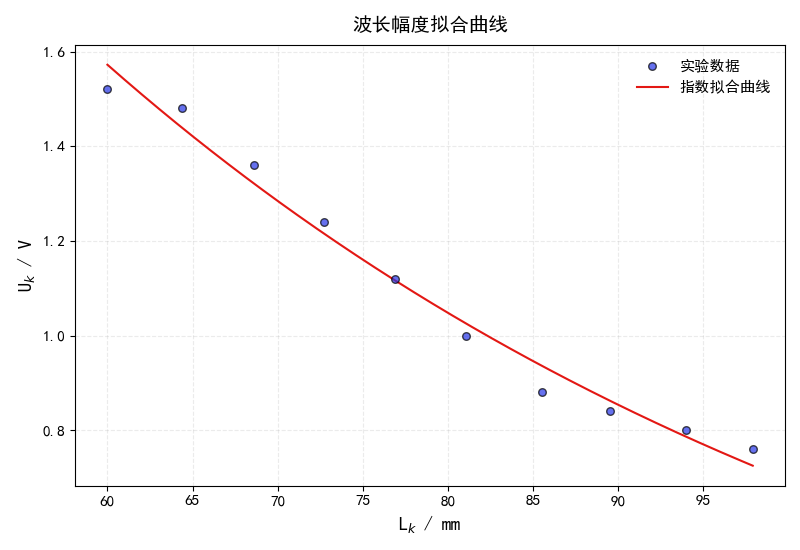
\includegraphics[width=0.75\textwidth]{Figure_3.png}
\end{figure}

拟合得到 $U=5.2415 e^{-0.0197L}-0.0400 \ \mathrm{V}$ 。计算得到当 $L > L_0 =-\frac{1}{0.0197}\ln \frac{U_0+0.04}{5.2415}=82.10\ \mathrm {mm}$ 时，声波信号的幅值衰减到 $1$ V 以下。

\subsubsection{用相位法测声速}

在用相位比较法时先将接收器与发射器约 $30\ \mathrm{mm}$以上的距离(距离太近波形会受发射器或接收器固定支架反射影响)，将示波器的显示调节为X-Y模式，适当改变示波器两个通道的Scale，利用李萨如图形来观察发射波与接收波的相位差。对于两个同频率简谐振动的合成，随着两者之间的相位差从 $0\sim\pi$ 变化，其李萨如图形由斜率为正的直线变为椭圆，再由椭圆变为斜率为负的直线，如 Figure 5 所示。记录游标卡尺上的读数时，应选择李萨如图形为直线时所对应的位置，每移动半个波长，就会重复出现正负交替的直线图形。

\begin{figure}[h]
  \centering
  \subfigure[]{
    \includegraphics[width=0.45\textwidth]{fig 5.jpg}
  }
  \subfigure[]{
    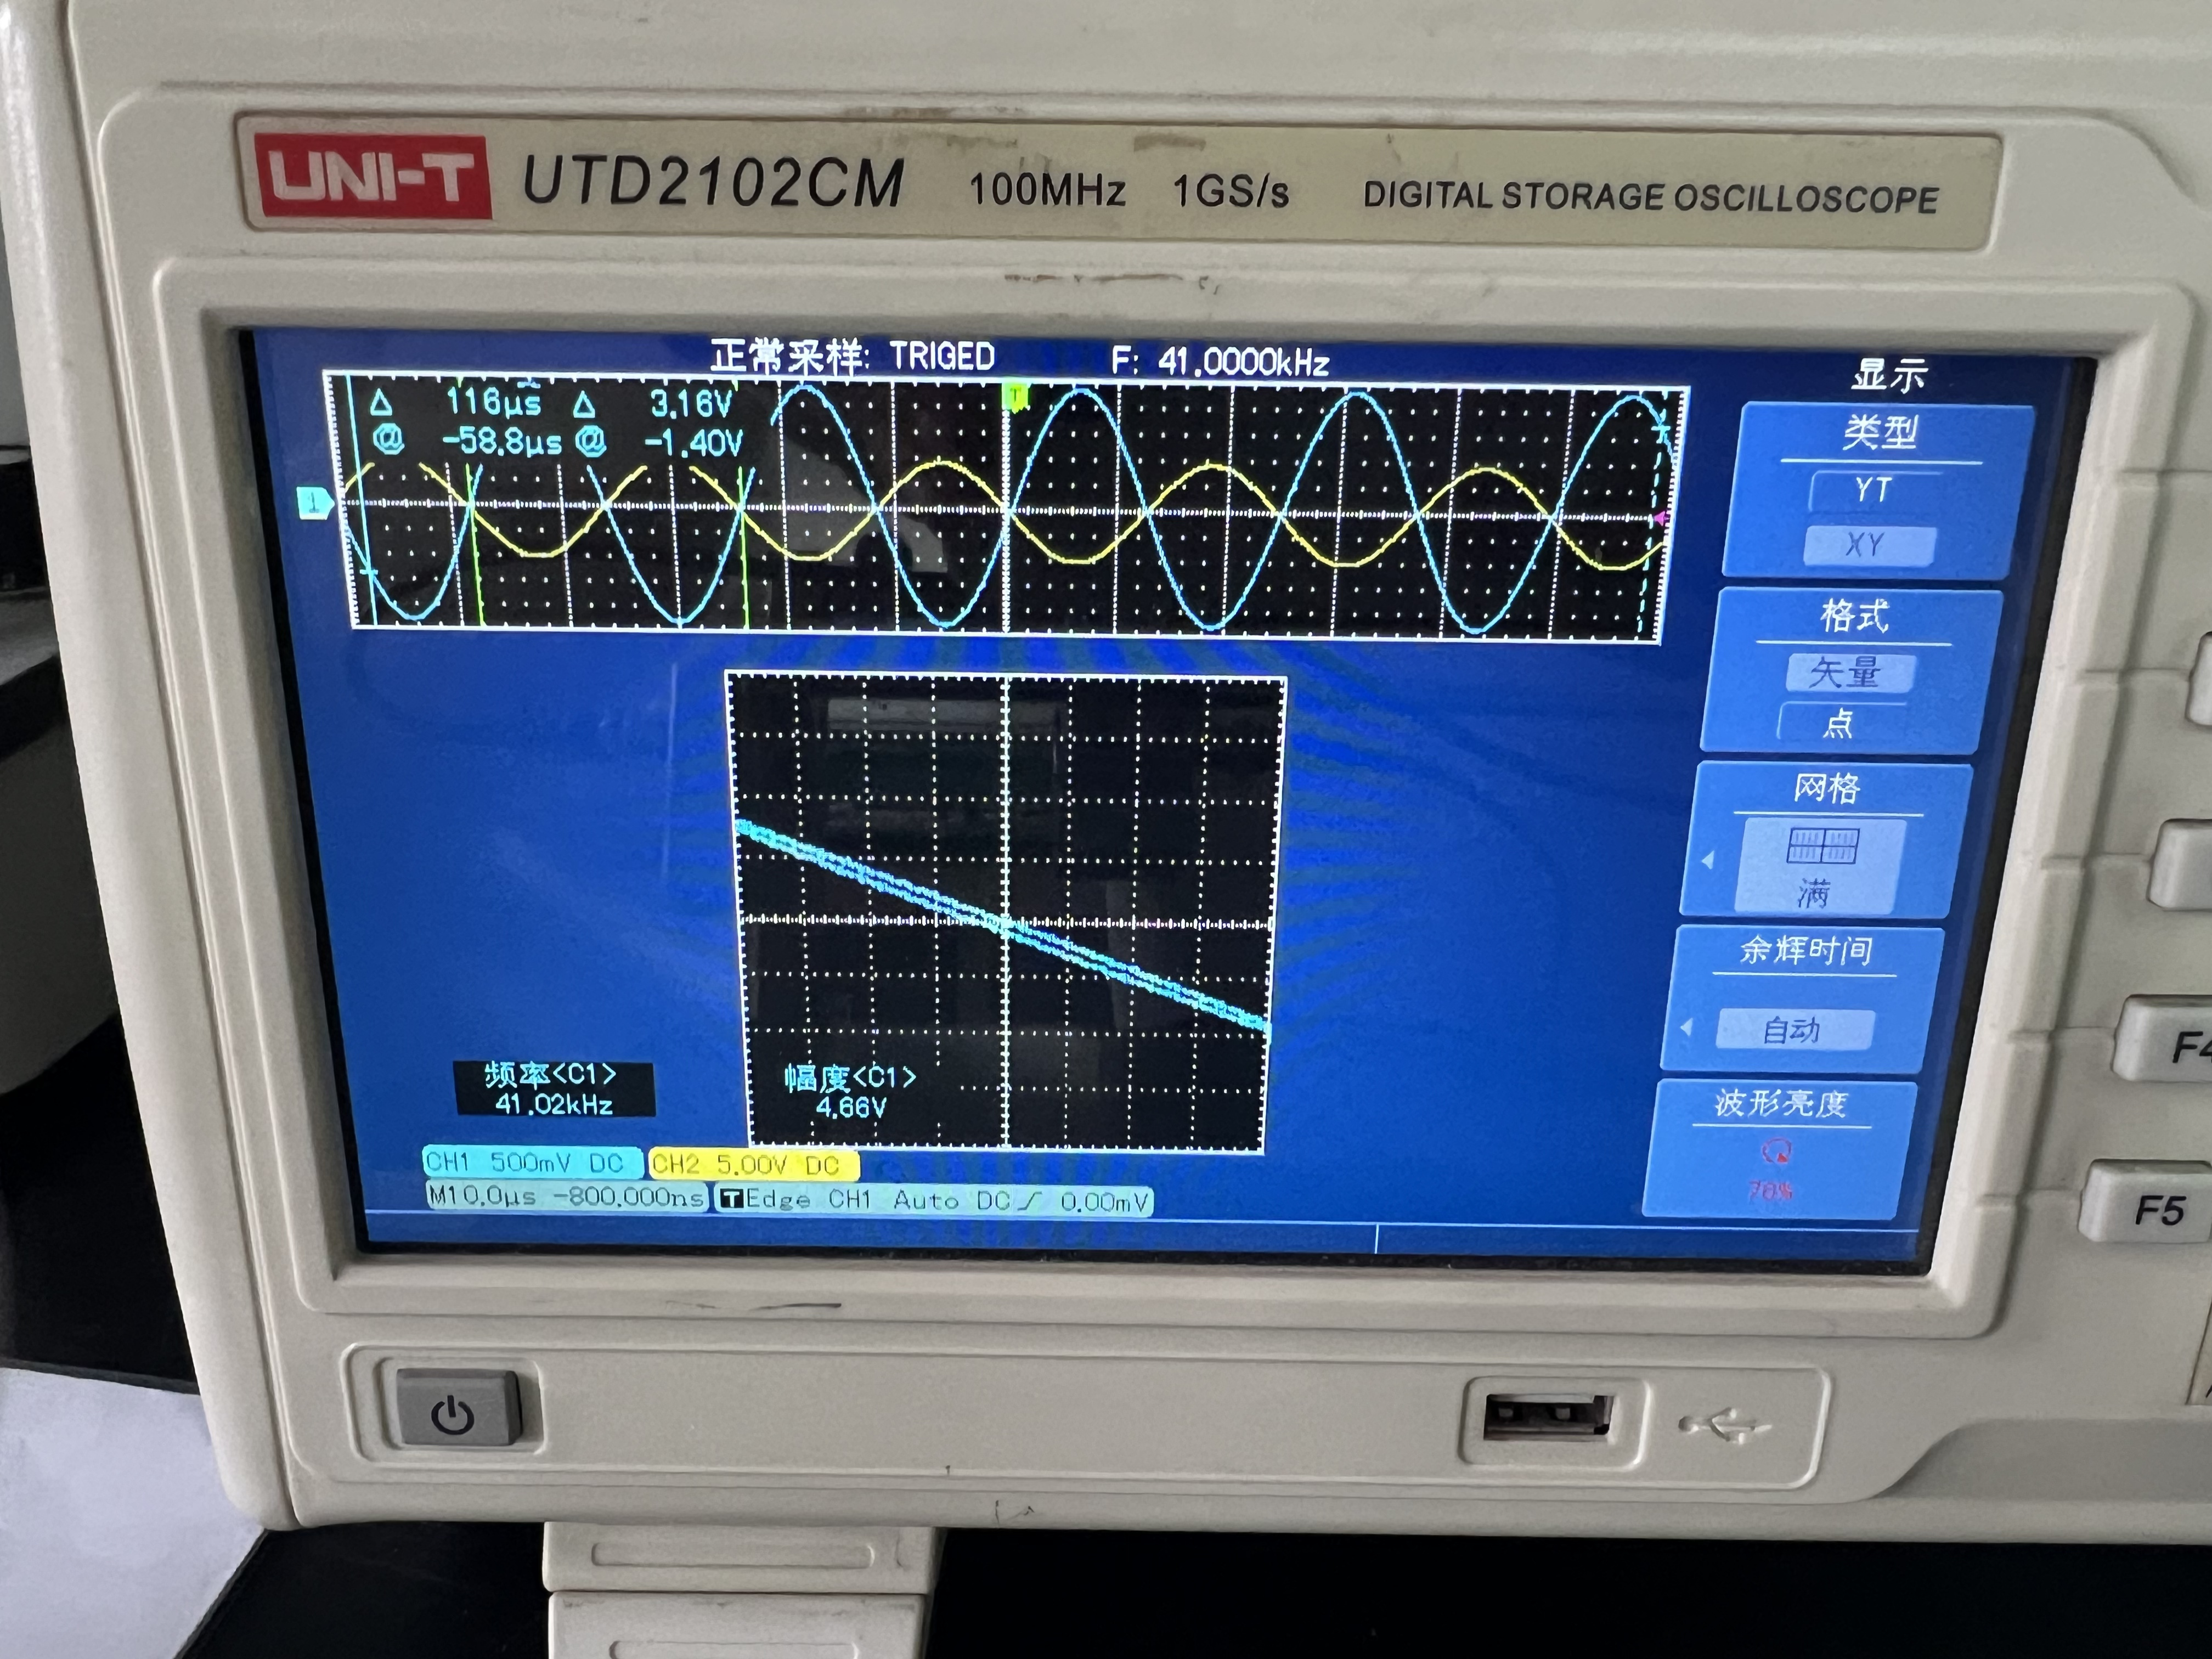
\includegraphics[width=0.45\textwidth]{fig6.jpg}
  }
  \caption{李萨如图}
  \label{fig:combined}
\end{figure}

\begin{table}[H]
\centering
\caption{相位法实验数据}
\vspace{2pt} 
\begin{minipage}{0.7\textwidth}
        \raggedleft
        $f= 40.9\ \mathrm{kHz}$
    \end{minipage}\\[2pt]
\small
\begin{tabular}{ccccccccccc}
\hline\hline
$k$ & 1 & 2 & 3 & 4 & 5 & 6 & 7 & 8 & 9 & 10 \\ 
$L_k$/mm & 34.27 & 38.49 & 42.64 & 46.84 & 51.08 & 55.30 & 59.49 & 63.73 & 67.95 & 72.24 \\ 
\hline\hline
\end{tabular}
\end{table}

计算得到声速为
\begin{equation}
    u=\frac{\sum_{k=1}^{5}(L_{k+5}-L_k)}{5\times 5}f=344.84 \mathrm{m/s}
\end{equation}

\subsection{时差法测声速}
将函数发生器的输出改为 “脉冲串” 模式，将猝发周期设为 100ms，循环数设为 5。连续移动接收端 A，记录发射信号和接收信号 如Figure 6 。记录接收端的位置 $L$，同时记录从示波器中发射与接收信号相应点的时差 $t$。

本次实验中测得，$L=39.69\ \mathrm {mm}$ ， $t=133\ \mathrm{\mu s}$， 计算得到声速为
\begin{equation}
    u=\frac{L}{t}=298.42\ \mathrm{m/s}
\end{equation}

\subsection{超声测距}
利用磁钢将挡板固定在移动接收端 A 前，将超声接收器的反射输出端口与示波器相连。移动挡板，同时记录挡板的位置 $L$ 与液晶屏上显示的距离，比较两者的数值。

本次实验中测得，$L=74.95\ \mathrm{mm}$，$t=508\ \mathrm{\mu s}$ 。取4.3.2测量结果，计算得到，4.3中带来误差的间隙长度为
\begin{equation}
    \Delta L=\frac{ut}{2}-L=12.64mm
\end{equation}

\end{document}